\documentclass{article}

\usepackage{graphicx}
\usepackage{tikz}
\usepackage{tikzsymbols}
\usetikzlibrary{calc,patterns,shapes.geometric}
\pagestyle{empty}
\usepackage[margin=0pt]{geometry}
\geometry{papersize={14in,12in}}

\def\centerarc[#1](#2)(#3:#4:#5){\draw[#1] ($(#2)+({#5*cos(#3)},{#5*sin(#3)})$) arc (#3:#4:#5);}

\begin{document}
	\begin{figure}
		\centering
		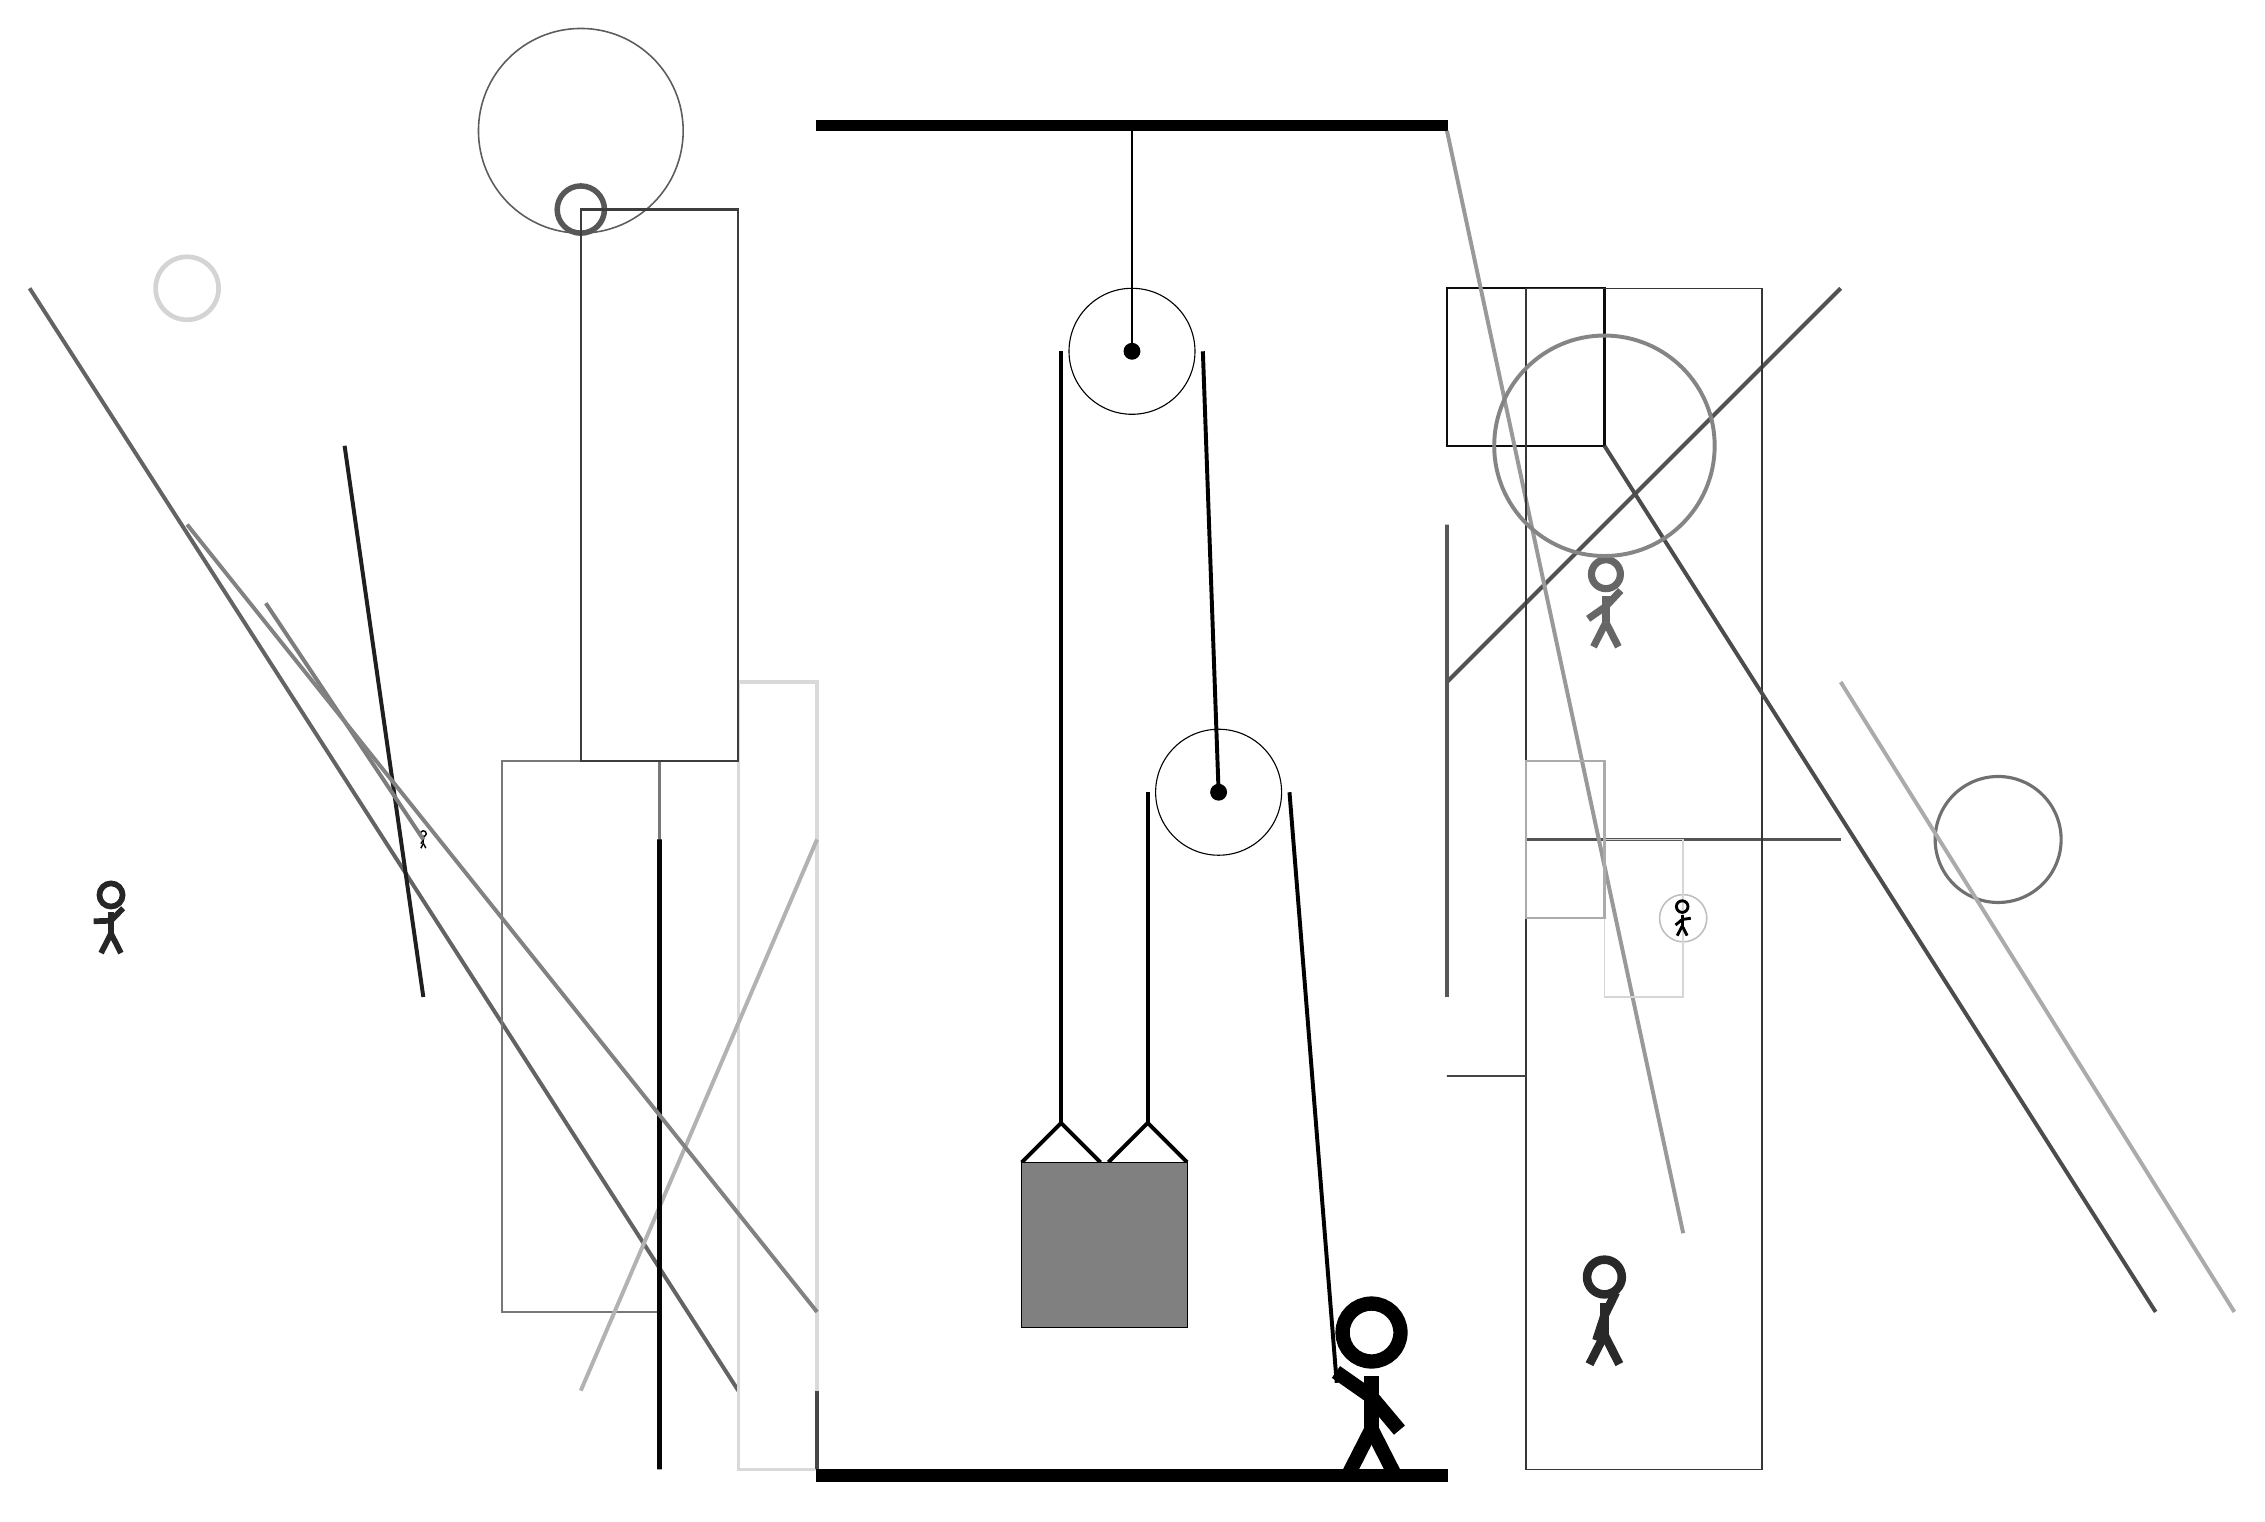
\begin{tikzpicture}
			%%%%% START %%%%%
			
			\draw[fill=black] (-2, 14) rectangle (6, 14.125);
			
			\draw (2, 11.2) circle (0.8);
			\draw[fill=black] (2, 11.2) circle (0.1);
			\draw[thick] (2, 11.2) -- (2, 14);
			
			\draw (3.1, 5.6) circle (0.8);
			\draw[fill=black] (3.1, 5.6) circle (0.1);
			
			\draw[line width = 0.5mm]  (0.6, 0.9) -- (1.1, 1.4) -- (1.6, 0.9);
			\draw[line width = 0.5mm]  (1.7, 0.9) -- (2.2, 1.4) -- (2.7, 0.9);
			\draw[fill=black!50] (0.6, 0.9) rectangle (2.7, -1.2);
			
			\draw[line width = 0.5mm] (1.1, 11.2) -- (1.1, 1.4);
			\centerarc[line width = 0.5mm](2, 11.2)(0:180:0.9);
			\draw[line width = 0.5mm] (2.9, 11.2) -- (3.1, 5.6);
			\draw[line width = 0.5mm] (2.2, 5.6) -- (2.2, 1.4);
			\centerarc[line width = 0.5mm](3.1, 5.6)(0:180:0.9);
			\draw[line width = 0.5mm] (4.0, 5.6) -- (4.6, -1.9);
			
			\draw[line width=0.5mm, color=black!61](-3, -2) -- (-12, 12);
			
			\draw[line width=0.5mm, color=black!88](-7, 3) -- (-8, 10);
			\draw[line width=0.3mm, color=black!53] (-4, 6) rectangle (-6, -1);
			\draw[line width=0.4mm, color=black!15] (-2, 7) rectangle (-3, -3);
			
			\node[line width=0.6mm, color=black!60] at (8, 8) {\Strichmaxerl[5][35][47]};
			\draw[line width=0.5mm, color=black!30](-5, -2) -- (-2, 5);
			\draw [line width=0.2mm, color=black!64](-5, 14) circle (1.3);
			
			\node[line width=0.2mm, color=black!99] at (-7, 5) {\Strichmaxerl[1][55][82]};
			\draw[line width=0.3mm, color=black!95] (6, 12) rectangle (8, 10);
			
			\draw[line width=0.7mm, color=black!98] (-4, -3) rectangle (-4, 5);
			\draw [line width=0.7mm, color=black!66](-5, 13) circle (0.3);
			
			\draw [line width=0.2mm, color=black!25](9, 4) circle (0.3);
			\draw[line width=0.5mm, color=black!67](7, 5) -- (11, 5);
			
			\draw[line width=0.5mm, color=black!51](-7, 5) -- (-9, 8);
			\draw [line width=0.4mm, color=black!56](13, 5) circle (0.8);
			\draw[line width=0.5mm, color=black!33](11, 7) -- (16, -1);
			
			\draw[line width=0.5mm, color=black!68](11, 12) -- (6, 7);
			\draw[line width=0.3mm, color=black!76] (-3, 13) rectangle (-5, 6);
			\draw[line width=0.5mm, color=black!40](6, 14) -- (9, 0);
			\draw[line width=0.5mm, color=black!72](-2, -3) -- (-2, -2);
			\draw[line width=0.2mm, color=black!16] (8, 5) rectangle (9, 3);
			
			\node[line width=0.4mm, color=black!84] at (8, -1) {\Strichmaxerl[6][72][64]};
			
			\draw[line width=0.2mm, color=black!79] (7, -3) rectangle (10, 12);
			\draw[line width=0.5mm, color=black!70](8, 10) -- (15, -1);
			\draw[line width=0.3mm, color=black!73] (6, 2) rectangle (7, 2);
			
			\draw[line width=0.3mm, color=black!33] (8, 4) rectangle (7, 6);
			\draw[line width=0.5mm, color=black!66] (6, 3) rectangle (6, 9);
			\draw [line width=0.6mm, color=black!17](-10, 12) circle (0.4);
			\draw [line width=0.5mm, color=black!48](8, 10) circle (1.4);
			\draw[line width=0.5mm, color=black!49](-2, -1) -- (-10, 9);
			\node[line width=0.7mm, color=black!100] at (9, 4) {\Strichmaxerl[2][40][8]};
			
			\node[line width=0.3mm, color=black!85] at (-11, 4) {\Strichmaxerl[4][2][46]};
			
			\node at (5, -2) {\Strichmaxerl[10][-35][-50]};
			
			\draw[fill=black] (-2, -3) rectangle (6, -3.15);
			
			%%%%% END %%%%%
		\end{tikzpicture}
	\end{figure}	
\end{document}